\chapter{Manufacturing Systems}
	
	To give a shape shape to a block of raw material, namely \textit{\textbf{workpiece}}, various methods can be used involving a different required number of \de{motion axis}:
	\begin{itemize}
		\item the \textbf{forming} processes that are based on the plastic deformation of the workpiece requires and usually requires the simultaneous motion of 1 motion axis; for shaping the workpiece it's not important the motion of the machine but usually only the force. In this course such manufacturing process is skipped because the motion planning and control is (usually) trivial;
		\item \textbf{subtractive} processes are based on the removal of material from the workpiece and usually requires the simultaneous motion of at least 2 axis and a rotation;
		\item we can add more material to the existing block using \textbf{additive manufacturing} techniques that, as for subtractive processes, requires at least 2.5 motion axis (2 synchronized plus one position axis that can be moved to ensure a particular position).
	\end{itemize}
	In subtractive/additive manufacturing there is a \de{tool} performing the process (such mills, polarized wires, extruding nozzles...) whose motion is performed by a synchronized action of two or more axes (typically in cartesian arrangement); the union of \textbf{trajectory} and \textbf{speed} of the tool represent it's \de{motion} that must be planned according to \textbf{geometry} (trajectory) and \textbf{process specifics} (for speed).
	
	
\section{Machining}
	
	The majority of products involves the \de{machining} process either directly or indirectly; machining involves a combination of linear and rotary motion and can be split in 3 main operational categories:
	\begin{itemize}
		\item \textbf{turning} where the workpiece is rotating and the tool is displacing; a good example of turning machining is the lathe (\textit{tornio});
		\item in \textbf{drilling} (performs holes) and \textbf{milling} (gives shape to a workpiece) the tool is rotating and there is a combined relative displacement between tool and workpiece.
	\end{itemize}
	The mechanism of \textbf{chip formation} (\textit{formazione di trucioli}) generated by this processes depends on multiple \textbf{tool parameters} such:
	\begin{itemize}
		\item the relative speed of the tool and the workpiece, namely the \textbf{cutting speed} $v$ (as the absolute value of the velocity vector);
		\item the cross section of the removed material.
	\end{itemize}
	This tool parameters strictly depends on the \textbf{machining parameters} as trajectory, rotation and translation speeds. Other relevant parameters to chose machining ones are the properties of the material used.
	
	Usually tool parameters are provided by the producer of the component and they so allows to compute the machining parameters as it will be shown in detail in the next sections.
	
	\subsection*{Turning}
		
		While dealing with \textbf{turning}, considering the scheme in figure \ref{fig:man:turning}, the main machining parameters that need to be calculated are the spindle speed, the feed rate and the spindle power.
		
		\begin{SCfigure}[2][bht]
			\centering 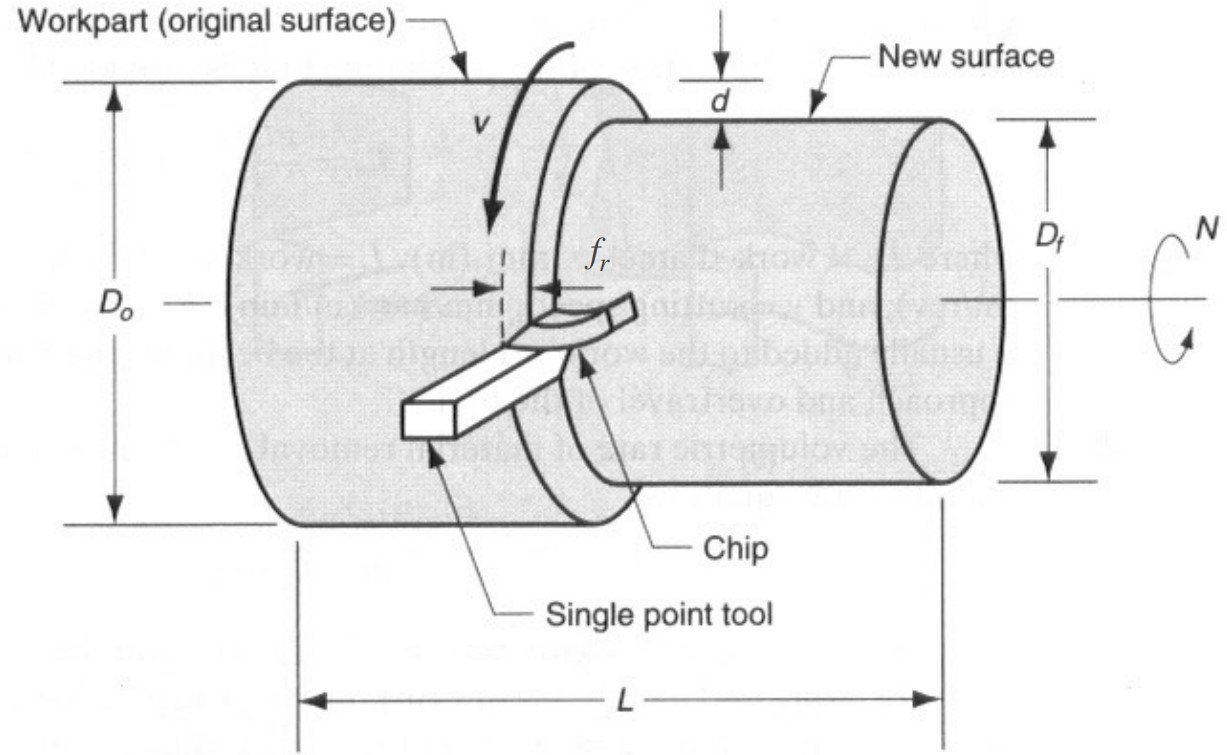
\includegraphics[width=7cm]{turning}
			\caption{main dimensions and parameters used for the calculation on turning's machining parameters.} \label{fig:man:turning}
		\end{SCfigure}
		
		Table \ref{tab:man:machiningparameters} contains a list of useful equations that can be used in order to compute the machining parameters; $N$ is the spindle rotation in revolution per minute and depends on the tangential velocity $v$ provided by the tool parameters; $D_0$ the external diameter of the shaft that has to be reduces to the value $D_f$; $f$ is the \textbf{feed rate}, measured in $mm/min$, is the velocity in the displacement along the axis of the tool tip.  The material removal rate $MRR$ determines the volume of the removed material in $cm^3/min$; this parameters is needed to estimate the power that the machine requires to perform the process.
		
		
		\begin{table}[bht]
			
			\tabrule
			\begin{center}
			\caption{formulas for machining parameters} \label{tab:man:machiningparameters}\vspace{2mm}
			\begin{tabular} {M{2.2cm} M{2.2cm} M{2.2cm} M{2.2cm} M{2.2cm}}
				\multirow{2}{*}{Parameter}  & \multirow{2}{*}{Turning} & \multirow{2}{*}{Drilling} & \multicolumn{2}{c}{Milling} \\ &&& side & face \\ \hline
				$v(m/min)$ & $\pi D_0 N$ & $\pi D N$ & $\pi D N$ \\
				$N(1/min)$ & $\frac{v}{\pi D_0}$ & $\pi D N$ & $\pi D N$ \\
				
			\end{tabular}	
			\end{center}
				
			\vspace{2mm}
			{\footnotesize Additional parameters are the specific power $p_s [W/cm^3]$ (depending on the material processed usually) }\\
			\tabrule 
		\end{table}
	
	\subsection*{Drilling and milling}
		Considering the schematic representation of the drilling process in figure \ref{fig:man:drilling},  the new parameters used to describe the process are the approach length $A$ as the dimension of the surface edge that's worked.
		
		\begin{SCfigure}[2][bht]
			\centering 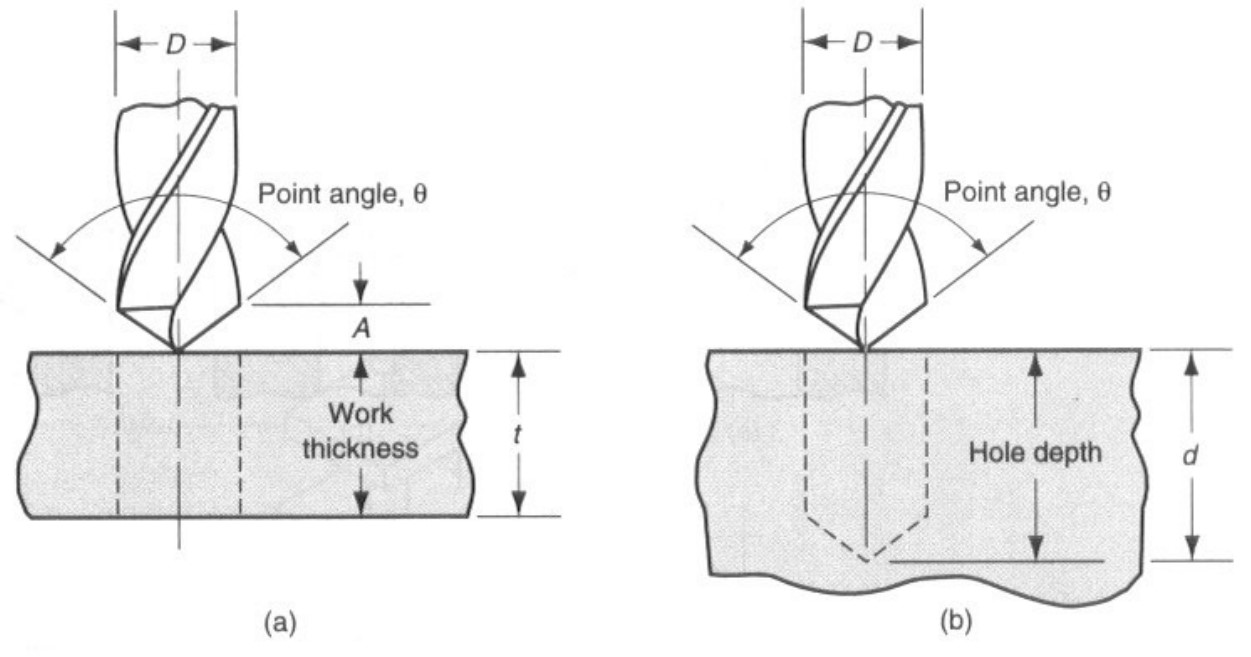
\includegraphics[width=9cm]{drilling}
			\caption{main dimensions and parameters used for the calculation on turning's machining parameters for drilling.} \label{fig:man:drilling}
		\end{SCfigure}
		
		Regarding milling (figure \ref{fig:man:milling}), such machining process can happen on the \textbf{side} or \textbf{face}: in the first case the rotary axis is parallel to the surface we are machining while for face milling the rotation axis is orthogonal.
		
		Typically in spindle machines the rotational speed goes from $5\,000 rpm$ up to $12\,000rpm$ (in extreme case up to $40\,000 rpm$).
			
	
		\begin{SCfigure}[2][bht]
			\centering 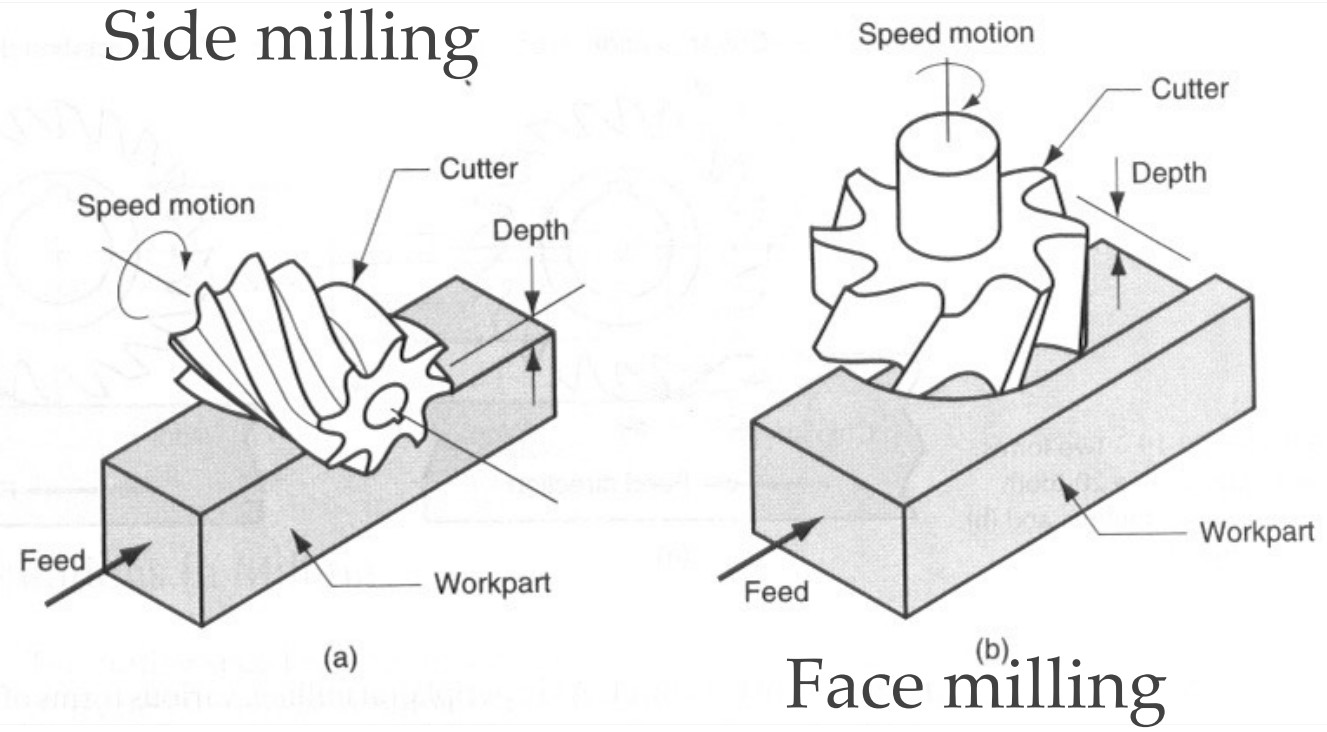
\includegraphics[width=9cm]{milling}
			\caption{main dimensions and parameters used for the calculation on turning's machining parameters for drilling.} \label{fig:man:milling}
		\end{SCfigure}

\section{Cutting economics}
	The \de{cost} of machining depends on a set of factor such:
	\begin{itemize}
		\item the labour as the hourly cost of trained personnel;
		\item the machinery purchase cost and it's lifetime span;
		\item the starting cost of raw material;
		\item the consumables such tools, fluids and other disposable fixtures.
	\end{itemize}
	Costs can either depend or not depend on process parameters; an example are tool that removes material: the wear of the flanks of the tool depends on the tangential velocity $v$  and the tool life $T$ following the \de{Taylor's} \textbf{tool wear law} 
	\begin{equation}
		v T^n = C
	\end{equation}
	where $n,C$ are function of the material and failure criteria. This means that 
	
	\begin{SCfigure}[2][bht]
		\centering 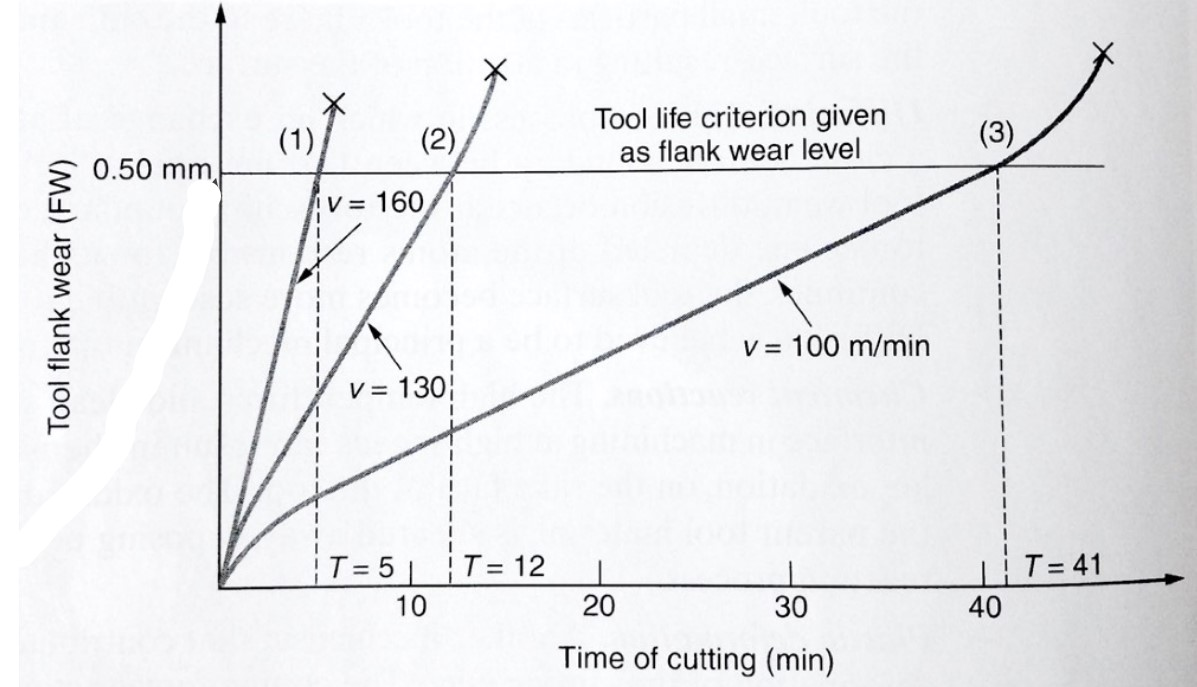
\includegraphics[width=6cm]{taylorslaw}
		\caption{example of diagram associated to the Taylor's tool wear  law.}
	\end{SCfigure}
	
	\subsection*{Economical model}
		Considering a cylindrical turning process for simplicity, we can regard the cost per piece $C_p$ as
		\[ C_p = C_m + C_s + C_l + C_t \]
		where $C_m$ is the machining, $C_s$ is the setup, $C_l$ the loading and $C_t$ the tooling costs. In particular the machining cost depends on the time for machining $T_m$ and the hourly costs related to labour $L_m$ and for the overhead $O_m$ (costs that you spend by still doing anything such rentals):
		\[ C_m = T_m (L_m + O_m) \]
		Similarly the loading and setup costs depends on the loading and setup time $T_l,T_s$: 
		\[ C_l = T_l  (L_m + O_m)  \hspace{2cm} C_s = T_s  (L_m + O_m)  \]
		
		\textbf{RIVEDERE UN ATTIMO QUESTA PARTE:} re-grinding tool
		
		$D_c$ is the depreciation as the price of the tool divided by the number of the allowable re-grinds; $N_p$ represent the number of pieces that can be manufactured by a tool.
		
\section{Machine tools}
	\subsection{Lathes}
		\de{Lathes} are machines used for performing turning process; \textbf{parallel} or \textbf{engine} lathes (figure \ref{fig:man:parallellathe}) are manual, while \textbf{CNC} ones are computer controlled and they can have a horizontal (single or multiple) spindle as well as vertical or with a sliding headstock (used for small components).
		
		\begin{SCfigure}[2][bht]
			\centering 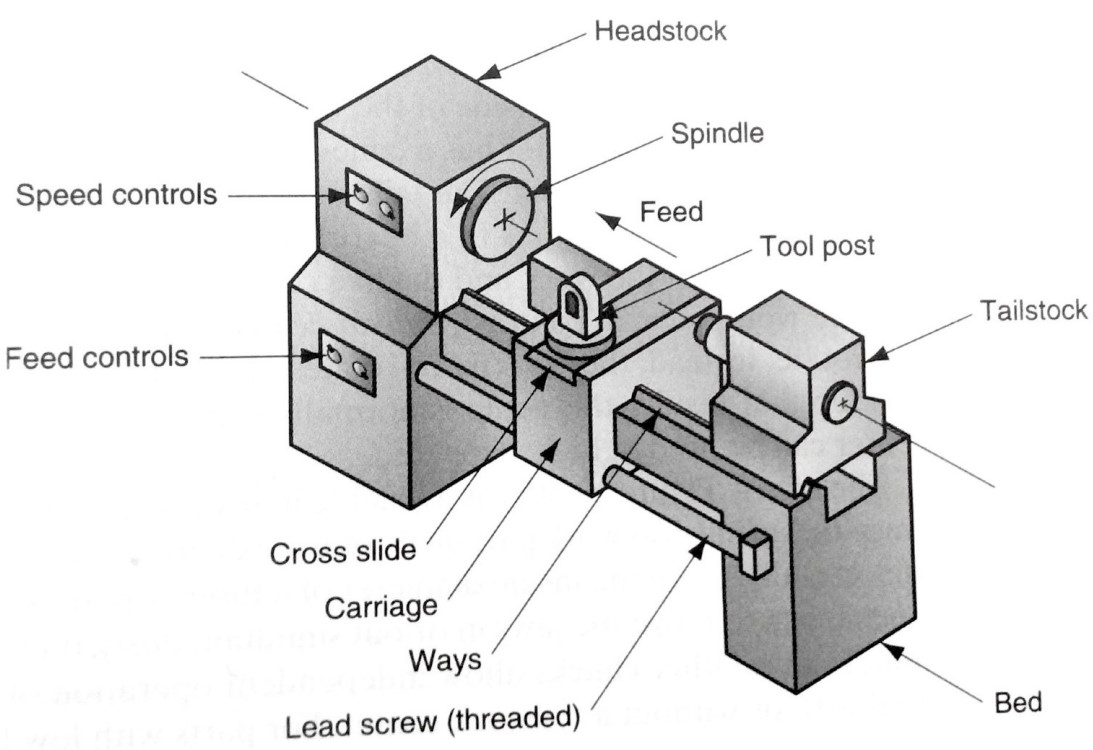
\includegraphics[width=7cm]{parallellathe}
			\caption{schematic representation of a parallel (engine) lathe.} \label{fig:man:parallellathe}
		\end{SCfigure}
		
		CNC lathes are similar to engine lathes but are enhanced by a computer-numerical-controller. The mechanical layout is arranged in order to allow automatic chip evacuation. Usually controllers handles 3 axis and a spindle (or more motion axis); they can also have a rotary tool determining so an \textbf{hybrid turning-milling} machine.
		
		They can dispose a \textbf{roller-turner} that automatically allows the machine to change the machining tool.
		
		Such machines can presents multiple tools and spindles and so with an increased complexity.\\
		Sliding headstock lathes presents a spindle that allows to axially move the component while the piecework is still rotating.
		
		While dealing with lathes, the most important \textbf{parameters} to determine are the turning diameter and length (maximum dimensions that can be machined), the slewing (dimensions of the raw material that can rotate on the spindle (but cannot be worked), the travels along the $z,x$ axis (but also other motion axis), the spindle speeds, the rapid speeds (maximum displacement speed along the axis, typically $10-40 m/min$) and spindle torque/power. Note that working with lower diameters, the required rotational speed is higher (while bigger components requires more torque) in order to maintain the tangential velocity constant.
		
		Usually graphs provided by manufacturer depends on the operating time \texttt{ED} as the values obtained considering, as example $100\%$ time work-load or $40\%$.
		
	\subsection{Milling machines}
		Milling machines presents a huge variety of architectures whose common denominator is the rotary tool. Spindles can be both horizontals or verticals and when more then 3 axis are moving we refer them to \textbf{milling centers} that are sub-categorized as  universal, pallet changes (the machine has two pallets: one that's objected of work and the other that can be accessed by the operator), travelling column. 
		
		Milling machines can be also realised using parallel kinematics (that's more complex to serial one) that realise faster movements for the same overall weight of the machine; a draw-back of this implementation is that the accuracy is not uniform in the whole working volume.
		
		\paragraph{Vertical and horizontal spindles} Vertical spindle machines are easier to implement, present an easy fixturing but has the problem of difficulties in the chip removal. Horizontal spindles presents a better chip disposal and allows for large travels with the draw-back of a more difficult fixture.
		
		\paragraph{Parameters} Parameters for milling machines are similar to the lathes, but comprehend also axes configurations and related travels.
		
\section{Automation}
	Tasks of a CNC machine tool is to convert a machining description into machining movement and then run machining commands with \textit{judgment} (level 4 on the yardstick table, page \pageref{tab:ind:amber}).
	
	Given the \textbf{part-program} containing the information about the process that has to be performed, such file is passed to the CNC (the computer numerical control) that gives instruction to both \textbf{drivers}, the electronic systems controlling position and motion of machining axis with sync, and \textbf{PLC} (\textit{programmable logic controller}, a separate hardware or a software in the same CNC machine), special controls that actuates supplementary axis (as safety doors or swingling arm for pallet change) that does take care on \textit{discrete} states (a door is open or closed, it doesn't matter it's trajectory nor motion).
	
	\subsection*{Linear axis control}
		
		
		
		
		
		
		
		
		
		